\documentclass[12pt, french]{article}

\usepackage{fancyhdr, fancybox, lastpage, makecell}
\usepackage[most]{tcolorbox}
\usepackage[a4paper, margin={0.3in, .75in}]{geometry}
\usepackage{wrapfig}
\pagestyle{fancy}
\renewcommand\headrulewidth{1pt}
\renewcommand\footrulewidth{1pt}
\fancyhf{}
\rhead{ \em{Zakaria Haouzan}}
\lhead[C]{\em{2ème année baccalauréat SM-X}}
\chead[C]{}
\rfoot[C]{}
\lfoot[R]{ \emph{Exercices Supplémentaires}}
\cfoot[]{\em{Page \thepage / \pageref{LastPage}}}


\newtcolorbox{Box2}[2][]{
                lower separated=false,
                colback=white,
colframe=white!20!black,fonttitle=\bfseries,
colbacktitle=white!30!gray,
coltitle=black,
enhanced,
attach boxed title to top left={yshift=-0.1in,xshift=0.15in},
title=#2,#1}


\begin{document}
\begin{center}
   \shadowbox {\bf{Décroissance Radioactive }}
\end{center}

\vspace{-0.2cm}
%%_________________________Exercice ! :"_________________________Exercice
%   \begin{center}
	   %\vspace{-0.6cm}
	%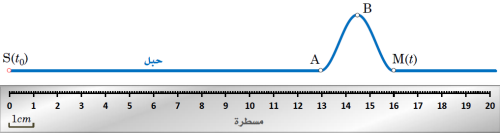
\includegraphics[width=0.6\textwidth ]{./img/Exercice01.png}
  %\end{center}



\begin{Box2}{\textbf{Exercice 1 :Le cobalt 60 }
	}
	Le cobalt $_{27}^{60}Co$ est un radionucléide émetteur $\beta^-$.

	\textbf{1. }Préciser la nature de la radioactivité $\beta^-$.
	
	\textbf{2. } Écrire l’équation de la réaction de désintégration du cobalt 60. Préciser les règles utilisées.

	\textbf{3. } L’activité A d’un échantillon est le nombre de désintégrations par seconde.

\textbf{3.1 }Sachant que cette activité A est proportionnelle au nombre N de noyaux non désintégrés qu’il contient, montrer que cette grandeur varie au cours du temps selon la loi $ln(\frac{A_0}{A}) = \lambda.t$

	\textbf{3.2 }Préciser le nom de la constante $\lambda$.

	\textbf{4. } Calculer la période du cobalt 60, sachant qu'au bout d'un an, l'activité a diminué de $12\%$.

	On donne : $_{28}Ni$ ; $_{26}Fe$ ; $_{29}Cu$

\end{Box2}


\begin{Box2}{\textbf{Exercice 2 : La radioactivité et la datation géologique}}
Lors de l’éruption d’un volcan il se forme des roches volcaniques qui contiennent parfois du potassium   $_{19}^{40}K$ radioactif, sa désintégration spontanée conduit à la formation de l’argon $_{18}^{40}Ar$.

\textbf{1. }Donner la composition du noyau du potassium $_{19}^{40}K$.

\textbf{2. }Écrire l’équation de la désintégration du noyau du potassium $_{19}^{40}K$ en précisant la nature de la particule émise.

\textbf{3. } Déterminer $\lambda$ la constante radioactive du potassium $_{19}^{40}K$, sachant que le temps de demi- vie de $_{19}^{40}K$ est $t_{1/2}=1,3.10^{9}ans$

\textbf{4. } Un échantillon de roches volcaniques formées à un instant considéré comme origine des temps $(t=0)$ contient $N_0$ noyaux du potassium $_{19}^{40}K$ et ne contient pas d’argon $_{18}^{40}Ar$.

L’analyse d’un même échantillon de ces roches à un instant t montre qu’il contient $N_k = 4,49.10^{19}$ noyaux de potassium $_{19}^{40}K$  et $N_{Ar} = 1,29.10^{17}$ noyaux d’argon $_{18}^{40}Ar$, $N_0=N_k + N_{Ar}$

-Déterminer la valeur de t l’âge des roches volcanique de l’échantillon.
\end{Box2}

\begin{Box2}{\textbf{Exercice 3 : Datation au carbone 14 }}
Lorsque, dans la haute atmosphère, un neutron appartenant au rayonnement cosmique rencontre
un noyau d’azote $^{14}_7N$, il donne naissance à du carbone 14, isotope de carbone $^{12}_6C$.

\textbf{1. }Écrire l’équation de la réaction en précisant la nature de la particule apparue avec le carbone 14.

\textbf{2. }Le noyau de carbone 14 se désintègre en émettant un rayonnement $\beta^-$ Écrire le bilan de cette réaction nucléaire.

\textbf{3. }Des végétaux absorbent le dioxyde de carbone de l’atmosphère provenant indifféremment du
carbone 14 et de carbone 12. La proportion de ces deux isotopes est la même dans les végétaux vivants
et dans l’atmosphère. Mais lorsque la plante meurt, elle cesse d’absorber le dioxyde de carbone ; le
carbone 14 qu’elle contient se désintègre alors, sans être renouvelé, avec une demi-vie $t_{1/2} = 5570ans$.

\textbf{3.1 } Quelle sera l’activité d’un échantillon de végétal au bout d’une durée $t = n.t_{1/2}$ après sa mort ?

\textbf{3.2 } On a comparé l’activité $a_1$ d’un échantillon de bois trouvé dans une tombe égyptienne en 1998 avec l’activité $a_2$ d’un échantillon de référence dont l’activité était $a_0$ en 1985. Le rapport est $\frac{a_2}{a_1} = 1,85$.

Calculer l’ordre de grandeur de la date de la coupe du bois trouvé dans la tombe
\end{Box2}

\begin{Box2}{Exercice 4 : Datation d’une nappe phréatique}
Le chlore 36 est créé régulièrement dans la haute atmosphère et se trouve dans l’eau. Il est radioactif
 $\beta^-$ . Les eaux de surface ont une teneur en chlore 36 constante malgré sa radioactivité. Leur contact
avec
l’atmosphère et les mouvements de l’eau permettent d’en garantir la teneur. Les nappes phréatiques
d’écoulement lent en sous - sol voient leur teneur en chlore 36 diminuer. Ainsi, un forage réalisé dans
une telle nappe indique que celle - ci ne contient plus que $33\%$ de chlore 36 par rapport à une eau
courante. La demi-vie du chlore 36 est $t_{1/2} = 3,0.10^4ans$.

1. Écrire l’équation nucléaire de radioactivité du chlore 36.

2. Calculer l’âge de la nappe d’eau trouver par forage.

3. Est-il possible d’utiliser le silicium 32 pour réaliser cette datation, sachant que sa demi-vie est
$t_{1/2}=6,5.10^2ans$
\end{Box2}
\begin{Box2}{Exercice 5 : La radioactivité au service de la médecine}
La médecine est l’un des domaines qui a connu l’application de la radioactivité en utilisant des noyaux
radioactifs pour diagnostiquer et traité des maladies, l’un des noyaux utilisés est le rhénium 186 dans
le but de soulager les malades atteints de polyarthrite rhumatoïde

Les données : La constante radioactive du rhénium $_{75}^{186}Re$ est $\lambda = 2,2.10^{-6}= 0,19jour^{-1}$

\textbf{1. }La désintégration d’un noyau de rhénium $_{75}^{186}Re$.

\textbf{1.1 }Donner la composition du noyau du rhénium $_{75}^{186}Re$.

\textbf{1.2 }La désintégration du noyau de rhénium $_{75}^{186}Re$ donne un noyau d’osmium $_{76}^{186}Os$.
Ecrire
l’équation de désintégration du rhénium et déterminer la nature de cette désintégration

\textbf{2. }Injection locale d’une solution contenant du rhénium 186.
Le produit injectable se présente sous la forme d’une solution contenue dans un flacon de volume $V_0= 10 mL$ ayant une activité $a_0 = 4.10^9Bq$ à la date $t=0$, c'est-à-dire à la sortie du laboratoire pharmaceutique.

\textbf{2.1 }Déterminer en jours la valeur de demi-vie $t_{1/2}$ du rhénium $_{75}^{186}Re$

\textbf{2.2 }Trouver, à l’instant $t_1 = 4,8jours$, le nombre $N_1$ de noyau de rhénium contenu dans le flacon

\textbf{3.2 } À l’instant $t_1$ on prélève du flacon de volume $V_0 = 10mL$ une injection de volume V contenant $N = 3,65.10^{13}$ noyaux de rhénium 186, on l’injecte à un malade dans l’articulation de l’épaule, trouver la valeur de V.


\end{Box2}

\begin{Box2}{Exercice 6 : Datation d’une roche volcanique }

	Le magma terrestre contient de potassium, dont l’un des isotopes, $^{40}K$, est radioactif. Dans $12\%$
des cas, celui - ci se désintègre en argon 40, un gaz. Lors d’une éruption volcanique, les roches en
fusion laissent échapper les gaz dans l’atmosphère. Une fois refroidies, les roches gardent l’argon 40
prisonnier. La mesure du rapport $\frac{N_{Ar}}{N_{K}}$ permet de déterminer l’âge de la roche. La demi-vie du potassium 40 est $t_{1/2} = 1,3.10^9ans$

\textbf{1. }Écrire l’équation nucléaire de désintégration du potassium 40.

\textbf{2. }En inspirant des lois de conservation, écrire la relation qui existe entre $N_{K_0}$ , $N_K$ et $N_{Ar}$, où $N_{K_0}$ est $N_K$ à t=0.

\textbf{3. } Rappeler la relation entre $N_K$ et t.

\textbf{4.} Exprimer le rapport Ar en fonction de t. $N_k$

\textbf{5.} Déterminer l’âge de la roche si le rapport précédent est égal à 0,033.

\end{Box2}
	%\vspace{2cm}
%\begin{center}
   %\Large{ \em{Exercices Supplémentaires}}
%\end{center}


%\vspace{-0.7cm}
%%_________________________Exercice 5 : _________________________Exercice
%\begin{Box2}{Exercice 5 :Les ondes sonores }
%4
%\end{Box2}
%%_________________________Exercice 6 : _________________________Exercice
%\begin{Box2}{Exercice 6 : échographie}
%6
%\end{Box2}

\end{document}
